\documentclass{standalone}
\usepackage{tikz}
\usetikzlibrary{patterns, positioning}
\usepackage[sfdefault]{ClearSans} %% option 'sfdefault' activates Clear Sans as the default text font
\usepackage[T1]{fontenc}

\begin{document}
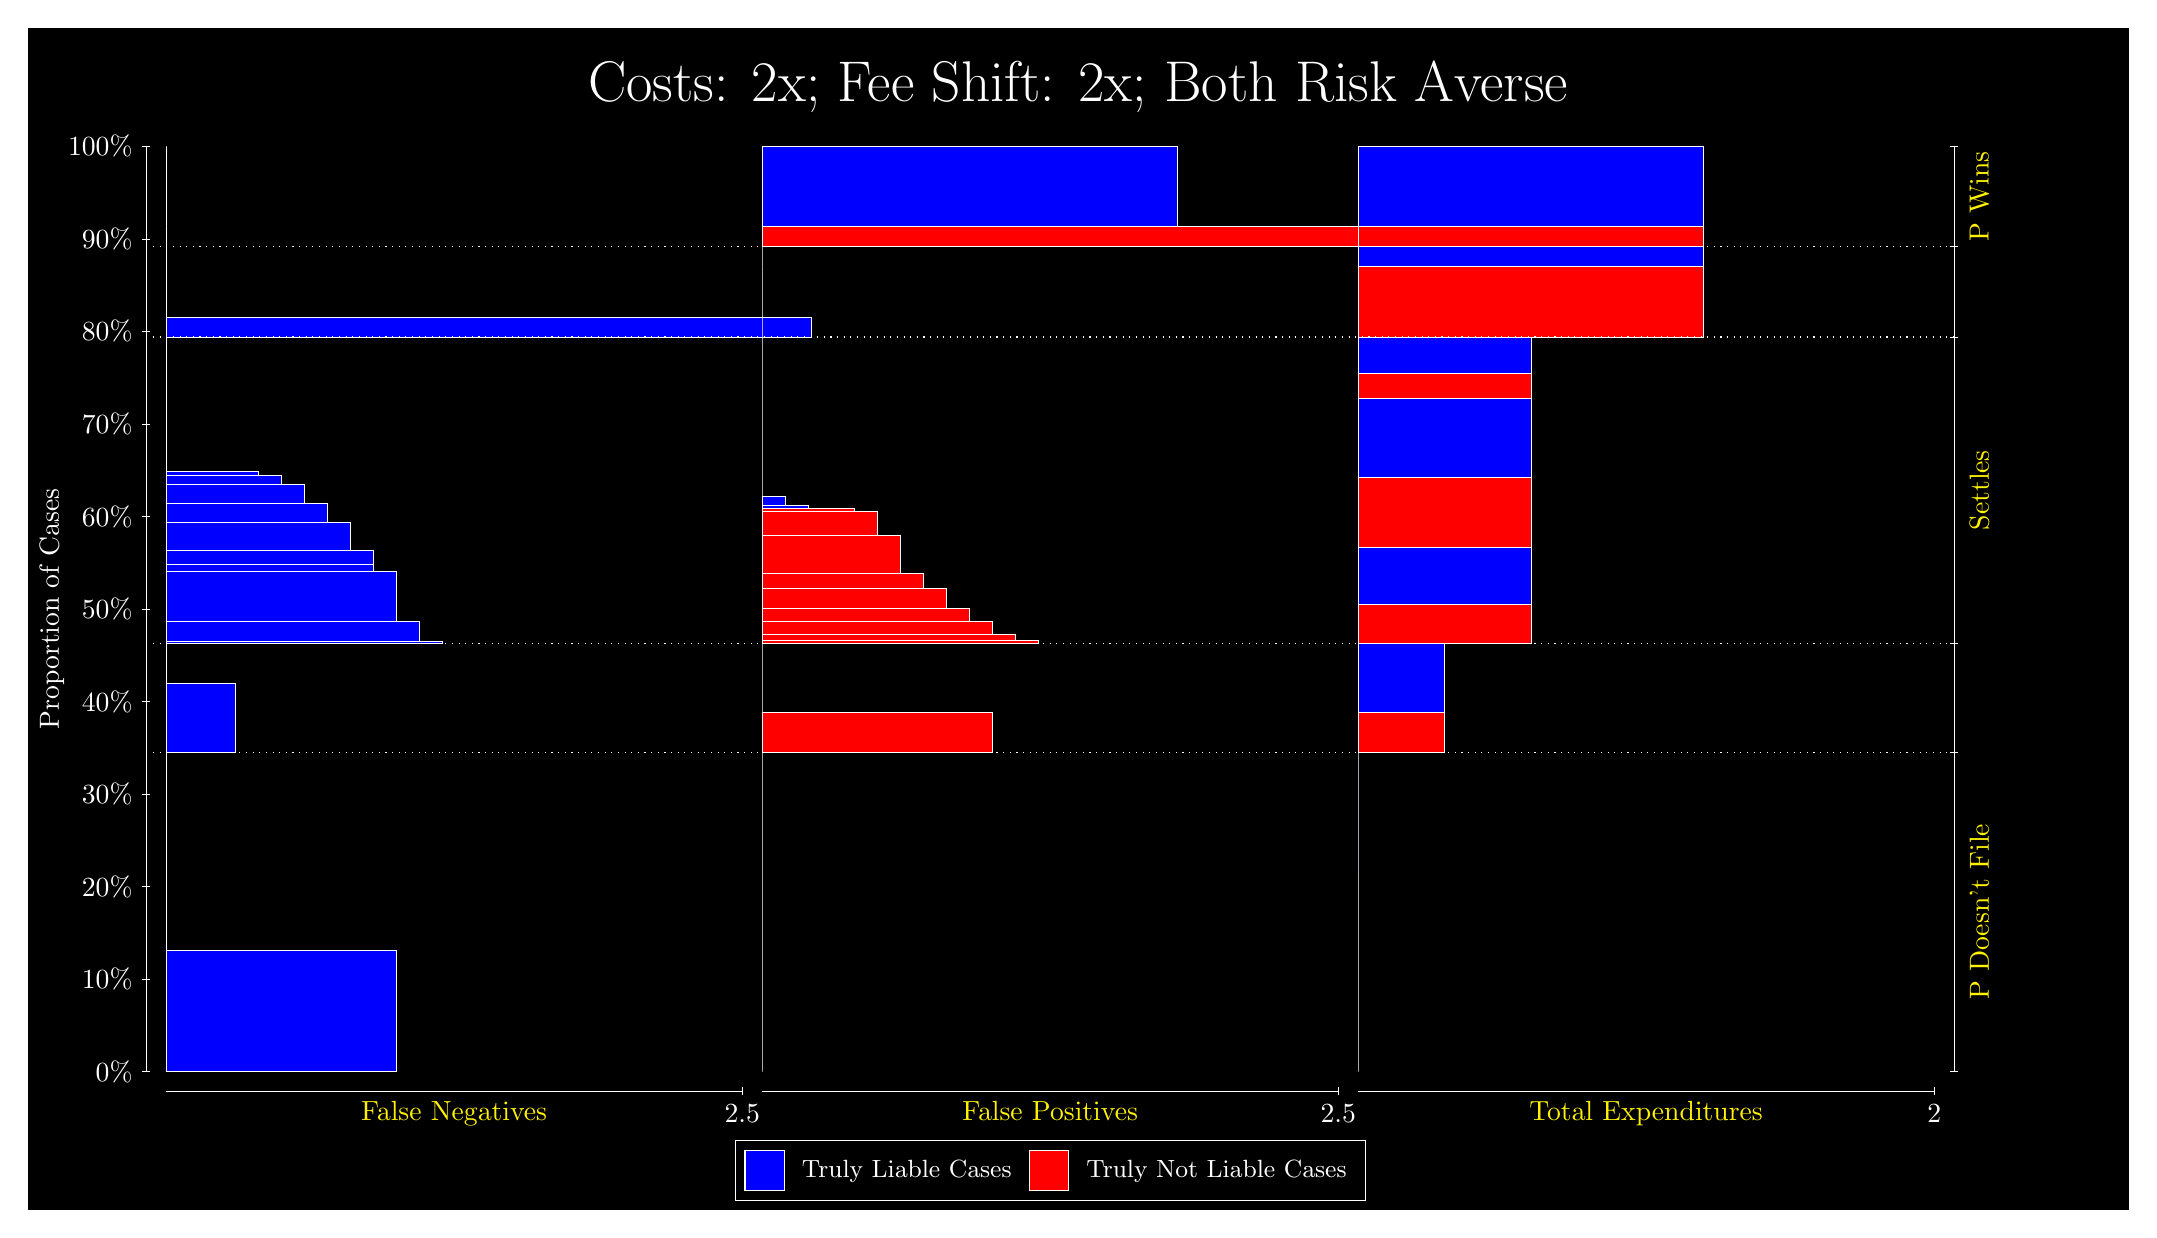
\begin{tikzpicture}
\draw[fill=black] (0,0) rectangle (26.667,15);
\draw[text=white] (0,13.5) rectangle (26.667,15) node[midway] {\huge Costs: 2x; Fee Shift: 2x; Both Risk Averse};
\draw[white, very thin] (1.5,1.75) -- (1.5,13.5);
\node[rotate=90, text=white, anchor=center] at (0.3, 7.625) {Proportion of Cases};
\draw[white, very thin] (1.45,1.75) -- (1.55,1.75);
\node[text=white, anchor=east] at (1.45, 1.75) {0\%};
\draw[white, very thin] (1.45,2.925) -- (1.55,2.925);
\node[text=white, anchor=east] at (1.45, 2.925) {10\%};
\draw[white, very thin] (1.45,4.1) -- (1.55,4.1);
\node[text=white, anchor=east] at (1.45, 4.1) {20\%};
\draw[white, very thin] (1.45,5.275) -- (1.55,5.275);
\node[text=white, anchor=east] at (1.45, 5.275) {30\%};
\draw[white, very thin] (1.45,6.45) -- (1.55,6.45);
\node[text=white, anchor=east] at (1.45, 6.45) {40\%};
\draw[white, very thin] (1.45,7.625) -- (1.55,7.625);
\node[text=white, anchor=east] at (1.45, 7.625) {50\%};
\draw[white, very thin] (1.45,8.8) -- (1.55,8.8);
\node[text=white, anchor=east] at (1.45, 8.8) {60\%};
\draw[white, very thin] (1.45,9.975) -- (1.55,9.975);
\node[text=white, anchor=east] at (1.45, 9.975) {70\%};
\draw[white, very thin] (1.45,11.15) -- (1.55,11.15);
\node[text=white, anchor=east] at (1.45, 11.15) {80\%};
\draw[white, very thin] (1.45,12.325) -- (1.55,12.325);
\node[text=white, anchor=east] at (1.45, 12.325) {90\%};
\draw[white, very thin] (1.45,13.5) -- (1.55,13.5);
\node[text=white, anchor=east] at (1.45, 13.5) {100\%};

\draw[white, very thin] (24.457,1.75) -- (24.457,13.5);
\draw[white, very thin] (24.407,1.75) -- (24.507,1.75);
\node[anchor=west] at (24.407, 1.75) {};
\draw[white, very thin] (24.407,5.8046) -- (24.507,5.8046);
\node[anchor=west] at (24.407, 5.8046) {};
\draw[white, very thin] (24.407,7.1887) -- (24.507,7.1887);
\node[anchor=west] at (24.407, 7.1887) {};
\draw[white, very thin] (24.407,11.079) -- (24.507,11.079);
\node[anchor=west] at (24.407, 11.079) {};
\draw[white, very thin] (24.407,12.227) -- (24.507,12.227);
\node[anchor=west] at (24.407, 12.227) {};
\draw[white, very thin] (24.407,13.5) -- (24.507,13.5);
\node[anchor=west] at (24.407, 13.5) {};

\draw[white, very thin, fill=blue] (1.75,1.75) rectangle (4.6775,3.2941);
\draw[white, very thin, fill=red] (1.75,3.2941) rectangle (1.75,5.8046);
\draw[white, very thin, fill=blue] (1.75,5.8046) rectangle (2.6283,6.6841);
\draw[white, very thin, fill=red] (1.75,6.6841) rectangle (1.75,7.1887);
\draw[white, very thin, fill=blue] (1.75,7.1887) rectangle (5.2631,7.2105);
\draw[white, very thin, fill=blue] (1.75,7.2105) rectangle (4.9703,7.467);
\draw[white, very thin, fill=blue] (1.75,7.467) rectangle (4.6775,8.0989);
\draw[white, very thin, fill=blue] (1.75,8.0989) rectangle (4.3848,8.1919);
\draw[white, very thin, fill=blue] (1.75,8.1919) rectangle (4.3848,8.3667);
\draw[white, very thin, fill=blue] (1.75,8.3667) rectangle (4.092,8.7262);
\draw[white, very thin, fill=blue] (1.75,8.7262) rectangle (3.7993,8.9699);
\draw[white, very thin, fill=blue] (1.75,8.9699) rectangle (3.5065,9.2064);
\draw[white, very thin, fill=blue] (1.75,9.2064) rectangle (3.2138,9.3226);
\draw[white, very thin, fill=blue] (1.75,9.3226) rectangle (2.921,9.3676);
\draw[white, very thin, fill=red] (1.75,9.3676) rectangle (1.75,11.079);
\draw[white, very thin, fill=blue] (1.75,11.079) rectangle (9.9471,11.332);
\draw[white, very thin, fill=red] (1.75,11.332) rectangle (1.75,12.227);
\draw[white, very thin, fill=red] (1.75,12.227) rectangle (1.75,12.481);
\draw[white, very thin, fill=blue] (1.75,12.481) rectangle (1.75,13.5);
\draw[white, very thin, fill=red] (9.3189,1.75) rectangle (9.3189,4.2605);
\draw[white, very thin, fill=blue] (9.3189,4.2605) rectangle (9.3189,5.8046);
\draw[white, very thin, fill=red] (9.3189,5.8046) rectangle (12.246,6.3093);
\draw[white, very thin, fill=blue] (9.3189,6.3093) rectangle (9.3189,7.1887);
\draw[white, very thin, fill=red] (9.3189,7.1887) rectangle (12.832,7.2207);
\draw[white, very thin, fill=red] (9.3189,7.2207) rectangle (12.539,7.3048);
\draw[white, very thin, fill=red] (9.3189,7.3048) rectangle (12.246,7.4674);
\draw[white, very thin, fill=red] (9.3189,7.4674) rectangle (11.954,7.6361);
\draw[white, very thin, fill=red] (9.3189,7.6361) rectangle (11.661,7.8904);
\draw[white, very thin, fill=red] (9.3189,7.8904) rectangle (11.368,8.0777);
\draw[white, very thin, fill=red] (9.3189,8.0777) rectangle (11.075,8.5621);
\draw[white, very thin, fill=red] (9.3189,8.5621) rectangle (10.783,8.8592);
\draw[white, very thin, fill=red] (9.3189,8.8592) rectangle (10.49,8.8999);
\draw[white, very thin, fill=blue] (9.3189,8.8999) rectangle (9.9044,8.9449);
\draw[white, very thin, fill=blue] (9.3189,8.9449) rectangle (9.6116,9.0611);
\draw[white, very thin, fill=blue] (9.3189,9.0611) rectangle (9.3189,11.079);
\draw[white, very thin, fill=red] (9.3189,11.079) rectangle (9.3189,11.973);
\draw[white, very thin, fill=blue] (9.3189,11.973) rectangle (9.3189,12.227);
\draw[white, very thin, fill=red] (9.3189,12.227) rectangle (17.516,12.481);
\draw[white, very thin, fill=blue] (9.3189,12.481) rectangle (14.588,13.5);
\draw[white, very thin, fill=red] (16.888,1.75) rectangle (16.888,4.2605);
\draw[white, very thin, fill=blue] (16.888,4.2605) rectangle (16.888,5.8046);
\draw[white, very thin, fill=red] (16.888,5.8046) rectangle (17.986,6.3093);
\draw[white, very thin, fill=blue] (16.888,6.3093) rectangle (17.986,7.1887);
\draw[white, very thin, fill=red] (16.888,7.1887) rectangle (19.083,7.6896);
\draw[white, very thin, fill=blue] (16.888,7.6896) rectangle (19.083,8.4019);
\draw[white, very thin, fill=red] (16.888,8.4019) rectangle (19.083,9.3027);
\draw[white, very thin, fill=blue] (16.888,9.3027) rectangle (19.083,10.306);
\draw[white, very thin, fill=red] (16.888,10.306) rectangle (19.083,10.615);
\draw[white, very thin, fill=blue] (16.888,10.615) rectangle (19.083,11.079);
\draw[white, very thin, fill=red] (16.888,11.079) rectangle (21.279,11.973);
\draw[white, very thin, fill=blue] (16.888,11.973) rectangle (21.279,12.227);
\draw[white, very thin, fill=red] (16.888,12.227) rectangle (21.279,12.481);
\draw[white, very thin, fill=blue] (16.888,12.481) rectangle (21.279,13.5);
\draw[white, dotted] (1.5,5.8046) -- (24.457,5.8046);
\draw[white, dotted] (1.5,7.1887) -- (24.457,7.1887);
\draw[white, dotted] (1.5,11.079) -- (24.457,11.079);
\draw[white, dotted] (1.5,12.227) -- (24.457,12.227);
\draw[white, very thin] (1.75,1.5) -- (9.0689,1.5);
\node[text=yellow, anchor=north] at (5.4094, 1.5) {False Negatives};
\draw[white, very thin] (9.0689,1.45) -- (9.0689,1.55);
\node[text=white, anchor=north] at (9.0689, 1.45) {2.5};

\draw[white, very thin] (9.3189,1.5) -- (16.638,1.5);
\node[text=yellow, anchor=north] at (12.978, 1.5) {False Positives};
\draw[white, very thin] (16.638,1.45) -- (16.638,1.55);
\node[text=white, anchor=north] at (16.638, 1.45) {2.5};

\draw[white, very thin] (16.888,1.5) -- (24.207,1.5);
\node[text=yellow, anchor=north] at (20.547, 1.5) {Total Expenditures};
\draw[white, very thin] (24.207,1.45) -- (24.207,1.55);
\node[text=white, anchor=north] at (24.207, 1.45) {2};

\node[text=yellow, centered, rotate=90] at (24.777, 3.7773) {P Doesn't File};

\node[text=yellow, centered, rotate=90] at (24.777, 9.1337) {Settles};

\node[text=yellow, centered, rotate=90] at (24.777, 12.863) {P Wins};

\draw (12.978300999999998,1.5) node[draw=none] (baseCoordinate) {};
\begin{scope}[align=center]
        \matrix[scale=0.5, draw=white, below=0.5cm of baseCoordinate, nodes={draw}, column sep=0.1cm]{
            \node[rectangle, draw, minimum width=0.5cm, minimum height=0.5cm, fill=blue] {}; &
            \node[draw=none, font=\small, text=white] (B) {Truly Liable Cases}; &
            \node[rectangle, draw, minimum width=0.5cm, minimum height=0.5cm, fill=red] {}; &
            \node[draw=none, font=\small, text=white] (B) {Truly Not Liable Cases}; \\
            };
\end{scope}

\end{tikzpicture}
\end{document}